% CV.tex
% !TEX TS-program = pdflatex
% !TEX encoding = UTF-8 Unicode
\documentclass[9pt, oneside, a4paper, titlepage]{extarticle}

\usepackage[most]{tcolorbox}
\usepackage{tikz}
\usepackage{graphicx}
\usepackage[]{geometry}
\usepackage{booktabs}
\usepackage{setspace}
\usepackage{multicol}
\usepackage{hyperref}
\geometry{
    a4paper,
    left=0.1cm,
    right=0.1cm,
    top=0.2cm,
    bottom=0.1cm
    }
    \renewcommand{\baselinestretch}{0.95}
    \definecolor{titleBack}{RGB}{0,128,255} % Blue
    
    \title{Tobias SAVARY}
    \date{}
    
    \begin{document}

    % Create the rectangle at the top of the CV 
    \tcbset{colframe=gray!95!black, colback=titleBack, arc = 3mm}
    
    \begin{tcolorbox}
        % Use to fill in the top
        \begin{minipage}{0.3\linewidth}
            %This is the place for the picture of your face
            % \hspace*{-0.3cm}\includegraphics[scale = 0.5]{img/TOBIAS SAVARY Photo identité Oct2020.jpg}
            \hspace*{1cm}
            \begin{tikzpicture} 

                \begin{scope}
                    \clip [rounded corners=.5cm] (0,0) rectangle coordinate (centerpoint) (3,4.5cm); 
                    \node [inner sep=0pt] at (centerpoint) {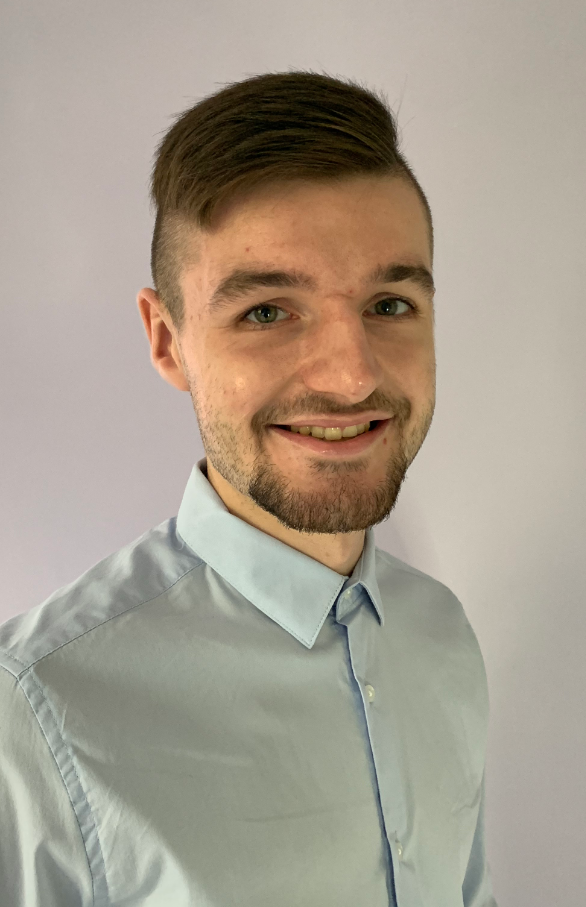
\includegraphics[width=3cm]{img/PhotoCV.png}}; 
                \end{scope}
            \end{tikzpicture}
        \end{minipage}%
        \hspace{1cm}%%
        \begin{minipage}{0.6\linewidth}
            \begin{center}
                \Huge{\textcolor{white}{Tobias SAVARY}} \\
                \vspace*{0.5cm}
                
                \Large{\textcolor{white}{Candidature pour le stage \emph{Data Analyst / \\ Développeur Costing Électricité (2024-115146)} \\ à partir de février 2025\\}}
                \vspace*{0.5cm}
                \Large{\textcolor{white}{\emph{Etudiant en Génie Informatique \\Université de Technologie de Compiègne (UTC) \\}}}
            \end{center}
        \end{minipage}%
    \end{tcolorbox}

    \tcbset{colframe=white, colback=white, arc = 2mm}
    \begin{tcolorbox}
        \vspace*{0.2cm}
        \hspace*{0.7mm}
        \begin{minipage}[t]{6.2cm}
            \begin{spacing}{0.95}
            \vspace*{-0.5cm}
            \begin{tcolorbox}[grow to left by = 0.6cm, colback = gray!25, colframe = white]
                % \section*{Profile}
                %     Here you can see my profile and I will complete it next time.
                
                \section*{\\Coordonnées}
                \hspace*{0.4cm}
                1 Allée du Tir à l'Arc

                \hspace*{0.4cm}
                \vspace*{0.2cm}
                60000 Beauvais\\
                \hspace*{0.4cm}
                Tel: +33 7 65 21 77 91\\
                \hspace*{0.4cm}
                Email: savarytobias@hotmail.com\\
                
                
                \vspace*{0.1cm}
                \hspace*{0.2cm} \href{www.linkedin.com/in/tobiassavary}{www.linkedin.com/in/tobiassavary}
                
                \vspace*{0.3cm}

                \hspace*{0.2cm} \href{https://github.com/TobiasInfo}{https://github.com/TobiasInfo}
                \vspace*{0.2cm}

                \section*{Programmation}
                \vspace*{0.2cm}
                \begin{multicols}{2}
                    \begin{itemize}
                        \item Python 
                        \item Numpy 
                        \item Pandas 
                        \item Scikit-learn
                        \item R
                        \item Power BI
                        \item SQL
                        \item Bash
                        \item C / C++
                        \item Java
                        \item React.js
                        %\item Java / Spring
                        % \columnbreak                    
                        %\item Dart / Flutter
                        %\item ARM
                        %\item HTML / CSS
                        %\item Express
                        \item \LaTeX
                    \end{itemize}
                    \end{multicols}
                    \vspace*{0.2cm}
                \section*{Compétences}

                \begin{itemize}
                    \vspace*{0.2cm}
                    \item Utilisation aisée des logiciels bureautiques (Word / Excel / Paint/ \\PowerPoint / \LaTeX \ldots)
                    \vspace*{0.2cm}
                    \item Utilisation aisée d’applications \\mobiles diverses
                    \vspace*{0.2cm}
                    \item Esprit d'équipe                    
                    % \vspace*{0.2cm}
                    \vspace*{0.2cm}
                    \item Communication
                    \vspace*{0.2cm}
                    \item Gestion de projet
                    \vspace*{0.2cm}
                    \item Gestion du temps
                    \vspace*{0.2cm}
                    \item Permis de conduire (A2 \& B)
                \end{itemize}


                \vspace*{0.2cm}
                
                \section*{Langues}
                \begin{itemize}
                    \item Français (langue maternelle)
                    \item Anglais (niveau européen C1)
                    \item Allemand (niveau européen A2)
                \end{itemize}
                \vspace*{0.51cm}

            \end{tcolorbox}
        \end{spacing}
        \end{minipage}
        \hspace*{0.4mm}
        \begin{minipage}[t]{12.8cm}
            \vspace*{-0.5cm}
            \begin{tcolorbox}[grow to right by = 0.6cm, colback = gray!25, colframe = white]
                \section*{Projets informatiques réalisés}

            %\begin{small}
                \begin{itemize}
                    \item Analyse comparative de modèles de machine learning pour les coûts d'assurance santé américains, incluant le nettoyage de données, l'EDA, et l'évaluation de performances avec Python (pandas, NumPy, Scikit-Learn)
                    \item Développement d'une solution de prise de décision pour un établissement de santé en utilisant SQL, Power BI, Bash, et Teradata, intégrant ETL, gestion de l'entrepôt de données, et création de tableaux de bord interactifs
                    \item Conception et réalisation d'une base de données pour une clinique vétérinaire
                    \item Réalisation de jeux de plateau en Python (scrabble, Futoshiki)
                    %\item Gestion d’ensembles mathématiques en Ocaml
                    %\item Traitement d’arbres phylogénétiques, décodage de message crypté, déplacement d’un robot, simplification de contours d’images en C
                    % \item Création d'un site web pour la gestion des embauches dans une entreprise. (gestion d'offres d'emplois, de candidatures, des permissions) en NodeJs, Express
                    % \item Développement d'une application de chat en temps réel utilisant Spring Boot, Java, React, REST et WebSocket.
                    \item Réalisation d'un site web pour la gestion des embauches (gestion d'offres d'emplois, de candidatures, des permissions) avec un chat intégré utilisant Spring Boot, Java, React, REST et WebSocket
                    \item Programmation orientée objet en C++ : conception et développement du jeu de société Machi Koro
                    \item Sécurisation d'une infrastructure sous Linux (permissions, services réseau\ldots)
                \end{itemize}
            %\end{small}
                \section*{Expériences professionnelles}
                \begin{itemize}
                    \item \textbf{2024 - Aujourd'hui }: Chargé d'accueil à la bibliothèque universitaire de l'UTC (accueil, promotion des ressources numériques, organisation d'évènements\ldots)
                    \item \textbf{2023 - 2024 }: Stage assistant ingénieur au sein d'IlemGroup de Plan-les-Ouates, Suisse (6 mois) : \\
                    - Développement de modules d'IlemERP \\
                    - Développement du tableau de bord de l'entreprise (Graphiques de chiffre d'affaires, Rapports RH, Liste des projets) avec Dart/Flutter et Java/Spring
                    \item \textbf{2022 - 2023 }: Chargé d'accueil à la bibliothèque universitaire de l'UTC
                    \item \textbf{2022 }: Stage d'excellence au sein du laboratoire INRIA 
                    de Grenoble (2 mois) : \\   - Réalisation d'une 
                    interface graphique pour un jeu d'apprentissage
                    du débogage
                    \item \textbf{2021}: Stages au sein des services départementaux de l’Oise (Agent administratif)
                    %\begin{itemize}
                    %    \item Agent administratif - Comité des Œuvres Sociales [COS]
                    %    \item Agent administratif polyvalent - Maison Départementale des Personnes Handicapées de l’Oise [MDPH]
                    %    \item Agent d’accueil - Agence Départementale d’Information sur le Logement de l’Oise [ADIL60]
                    %\end{itemize}
                    %\item \textbf{2017}: Stage d’observation en informatique au sein de la Direction Numérique du Conseil Départemental de l'Oise
                    
                    %\item \textbf{2017-2022}: Garde d’enfants et cours particuliers
                \end{itemize}

                \section*{Diplômes et formations }
                \begin{itemize}
                    \item \textbf{2024 - Aujourd'hui }: Etudiant en double diplôme de master parcours apprentissage et optimisation des systèmes complexes à l'UTC
                    \item \textbf{2022 - Aujourd'hui }: Etudiant en $3^{e}$ année de cycle ingénieur Génie Informatique filière intelligence artificielle et science des données à l'UTC - \emph{GPA: 5/5}        
                    \item \textbf{2024 }: Test d'anglais Linguaskill Anywhere (173/180 - Niveau B2)
                    \item \textbf{2020-2022 }: Formation préparatoire intégrée au réseau d’écoles d’ingénieurs Polytech, adossée à la licence du parcours "Mathématiques et Informatique" de l’Université Grenoble Alpes [UGA], dont les enseignements transverses (Anglais, gestion de projet, exploration professionnelle\ldots).\\\emph{Classement: 120ème sur 1 564 étudiants}
                    % \item \textbf{2020 }: Baccalauréat (Série S – Section Européenne Anglais - Mention bien)                 
                   % \item \textbf{2017}: Diplôme National du Brevet (Mention très bien)
                \end{itemize}
                \section*{Activités et intérêts}

                \begin{itemize}
                    \item Participation aux manifestations de communication (Journées Portes Ouvertes, Journée du lycéen, présentation de formations)
                    \item Cyclisme : participation à divers évènements et rencontres sportives
                    \item Natation, Badminton, Tennis de Table
                    
                \end{itemize}
                    
            \end{tcolorbox}
        \end{minipage}
    \end{tcolorbox}
\end{document}